\clearpage
\section{Methode}\label{sec:Methode}
Um die Performance der drei Mesh Stacks zu vergleichen wurde ein einheitliches Benchmark Konzept erarbeitet. Dieses definiert die Mesh Parameter, Testumgebungen, den Ablauf sowie sämtliche Messgrössen und Messreihen.

\subsection{Messablauf}
Für den Vergleich der 3 Mesh Netzwerkstacks Bluetooth Mesh (BT Mesh), Thread und Zigbee wird ein vom Mesh Protokoll unabhängiges Testkonzept umgesetzt welches in der Abbildung \ref{fig:KonzeptschemaTestablauf} als Konzeptschema dargestellt ist. Die Benchmark Slave Nodes (BSN) in der Abbildung als Sensoren und Aktoren mit unterschiedlichen Funktionalitäten dargestellt, bilden zusammen mit dem Benchmark Master Node (BMN) das zu testende Mesh Netzwerk. Innerhalb des Netzwerks wird dessen Organisation vom jeweiligen Protokoll sichergestellt. Das Testnetzwerk soll ein realitätsnahes Netzwerk nachbilden. Beispielsweise wird eine Hausautomation in einem Einfamilienhaus als Referenz angenommen in welchem jeweils nur gewisse Nodes untereinander Applikationsdaten austauschen. Ein Lichtschalter kommuniziert nur mit einer Lichtquelle und umgekehrt. Der selbe Lichtschalter tauscht jedoch keine Applikationsdaten mit dem Temperatursensor aus. Trotzdem bilden die Nodes zusammen ein Mesh Netzwerk.\\

Die Benchmark Management Station (BMS) welche mit dem BMN via USB/UART kommuniziert, ist zuständig für die Verwaltung und Verarbeitung der Benchmarks. Während eines Benchmark Prozesses sollen sämtliche Messungen jedoch unabhängig von der BMS durchgeführt werden damit allfällige Latenzzeiten der USB/UART Verbindung die Resultate nicht verfälschen.

\begin{figure}[h]
	\centering
	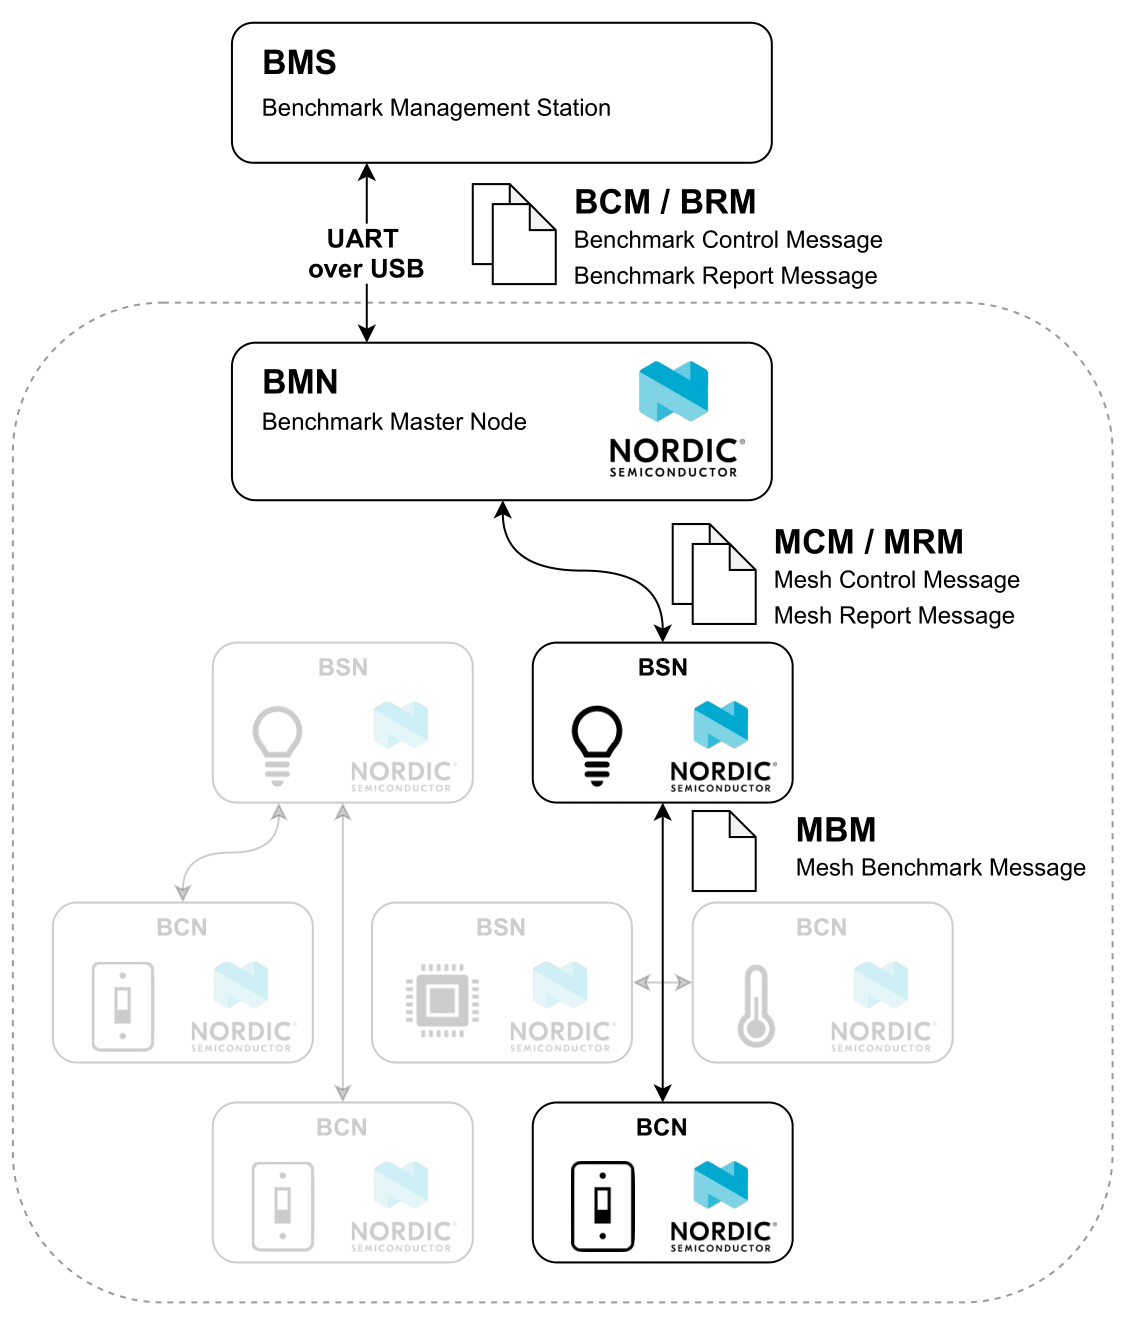
\includegraphics[width=0.55\textwidth]{graphics/Mesh_Testkonzeptschema.png}
	\caption{Konzeptschema Testablauf}
	\label{fig:KonzeptschemaTestablauf}
\end{figure}

\newpage
\subsection{Messaufbau}
Unterschiedliche Testumgebungen sollen die Benchmarks und schlussendlich den Vergleich der 3 Mesh Protokolle aussagekräftiger machen. Nachfolgende Umgebungen mit den entsprechenden Eigenschaften sollen getestet werden. Die Abbildungen zu den Testumgebungen zeigen jeweils die Platzierung der Nodes sowie deren Funktion und Gruppen Zugehörigkeit. Die Farbe Grün identifiziert den Node als Client Node während Blau für einen Server Nodes steht. Die Nummerierung zeigt welcher Node zu welcher Adressgruppe gehört. Ein Client Node in Gruppe 1 sendet jeweils Nachrichten zu allen Server Nodes in der selben Gruppe. 
\newline

\paragraph{Labor}
\begin{wrapfigure}{r}{0.6\textwidth}
	\centering
	\vspace{-20pt}
	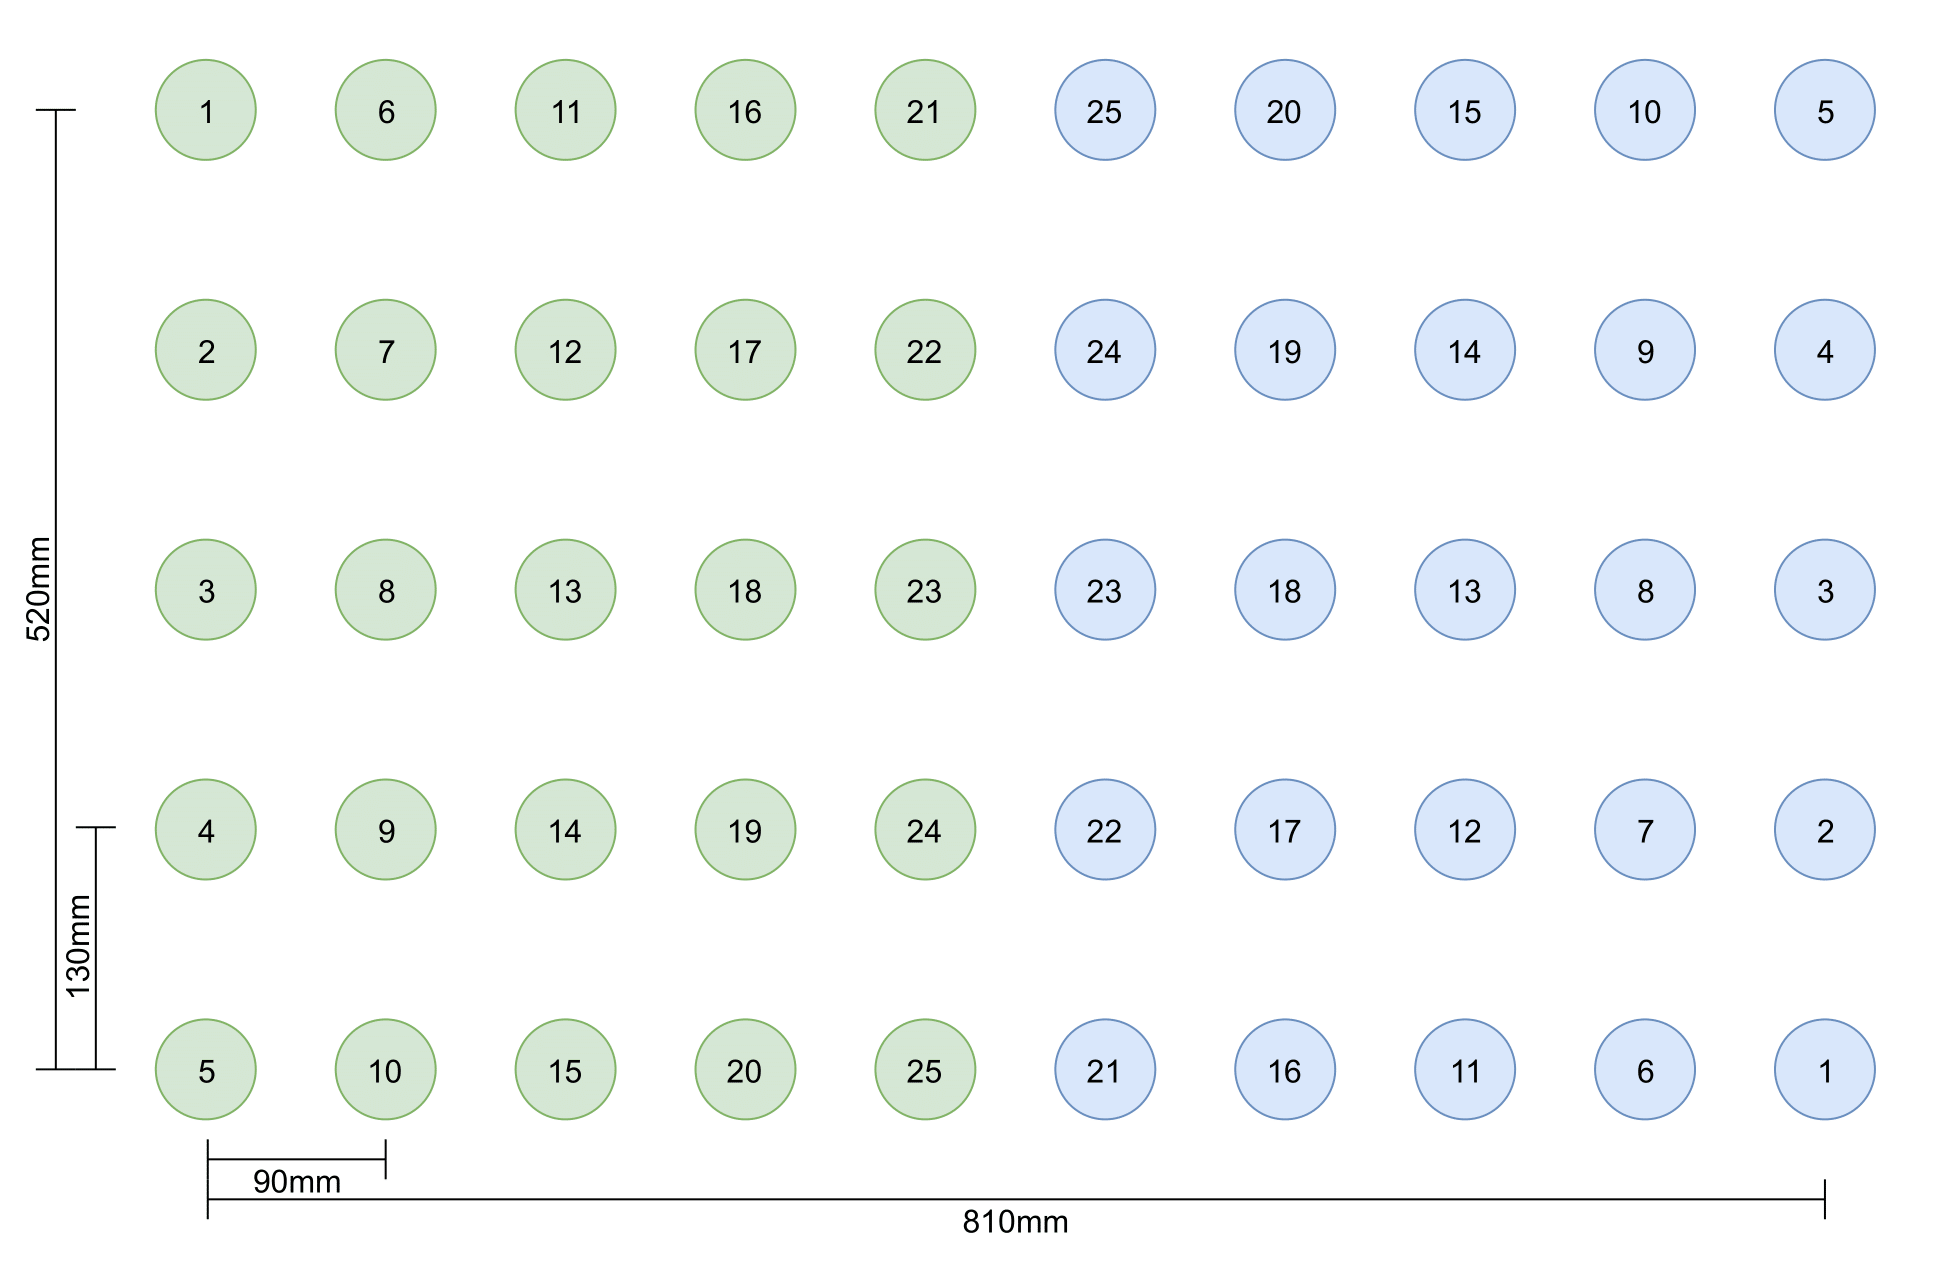
\includegraphics[width=0.6\textwidth]{graphics/Testaufbau_Labor.png}
	\caption{Testaufbau Labor}
	\label{fig:TestaufbauLabor}
	\vspace{-10pt}
\end{wrapfigure}
Der Laboraufbau ist ein Extremtest welcher die Leistungsgrenzen der Protokollstacks ausloten soll. Dabei werden die Nodes auf einem Raster gemäss Abbildung \ref{fig:TestaufbauLabor} angeordnet. Die genauen Abmessungen sind der Abbildung zu entnehmen.
\vspace{40mm}

\paragraph{Einfamilienhaus}
\begin{wrapfigure}{r}{0.6\textwidth}
	\centering
	\vspace{-105pt}
	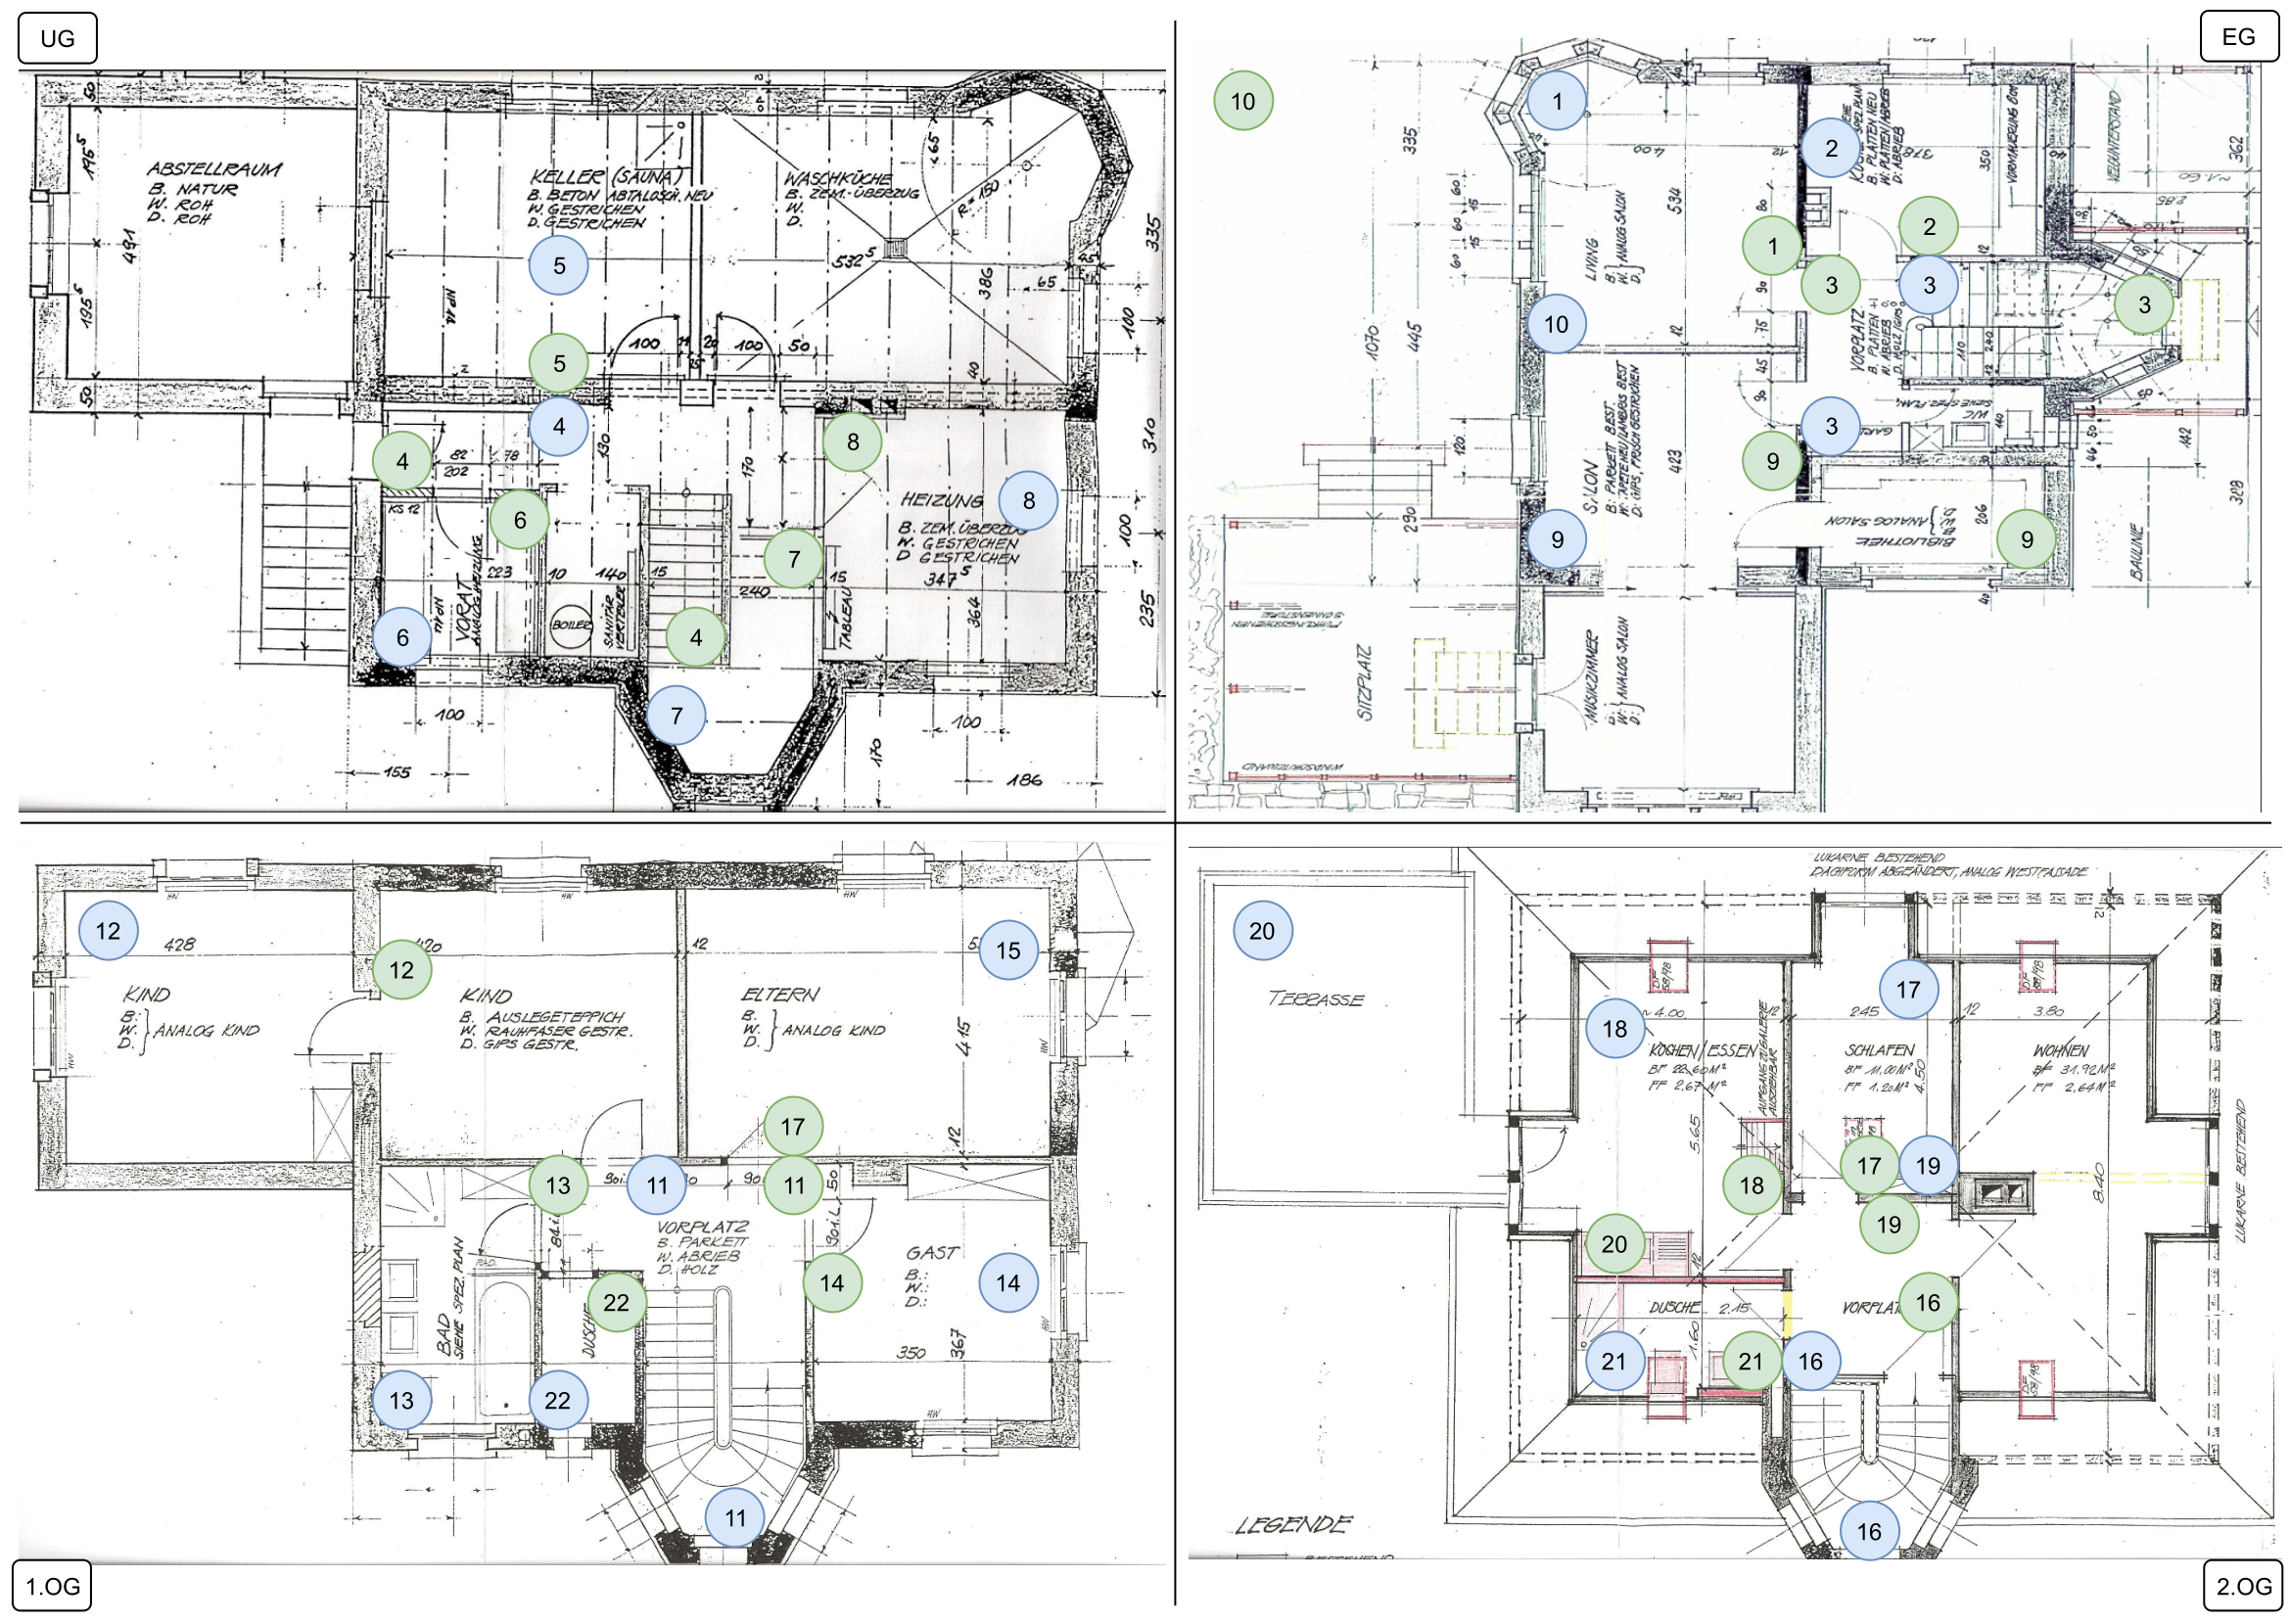
\includegraphics[width=0.6\textwidth]{graphics/Plan_Haus_Raffi.png}
	\caption{Platzierung der Nodes im Einfamilienhaus}\label{fig:Messumgebung2Einfamilienhaus}
	\vspace{-50pt}
\end{wrapfigure}
Die Testgeräte werden in einem Einfamilienhaus installiert und repräsentieren damit eine flächendeckende Heim-Automatisierung. Folgende Eingenschaften soll diese Messung abdecken:

Die Abbildung \ref{fig:Messumgebung2Einfamilienhaus} zeigt den Schnitt des Einfamilienhauses in welchem der Benchmark durchgeführt wurde.

\newpage
\paragraph{Wohnung}
\begin{wrapfigure}{r}{0.6\textwidth}
	\centering
	\vspace{-80pt}
	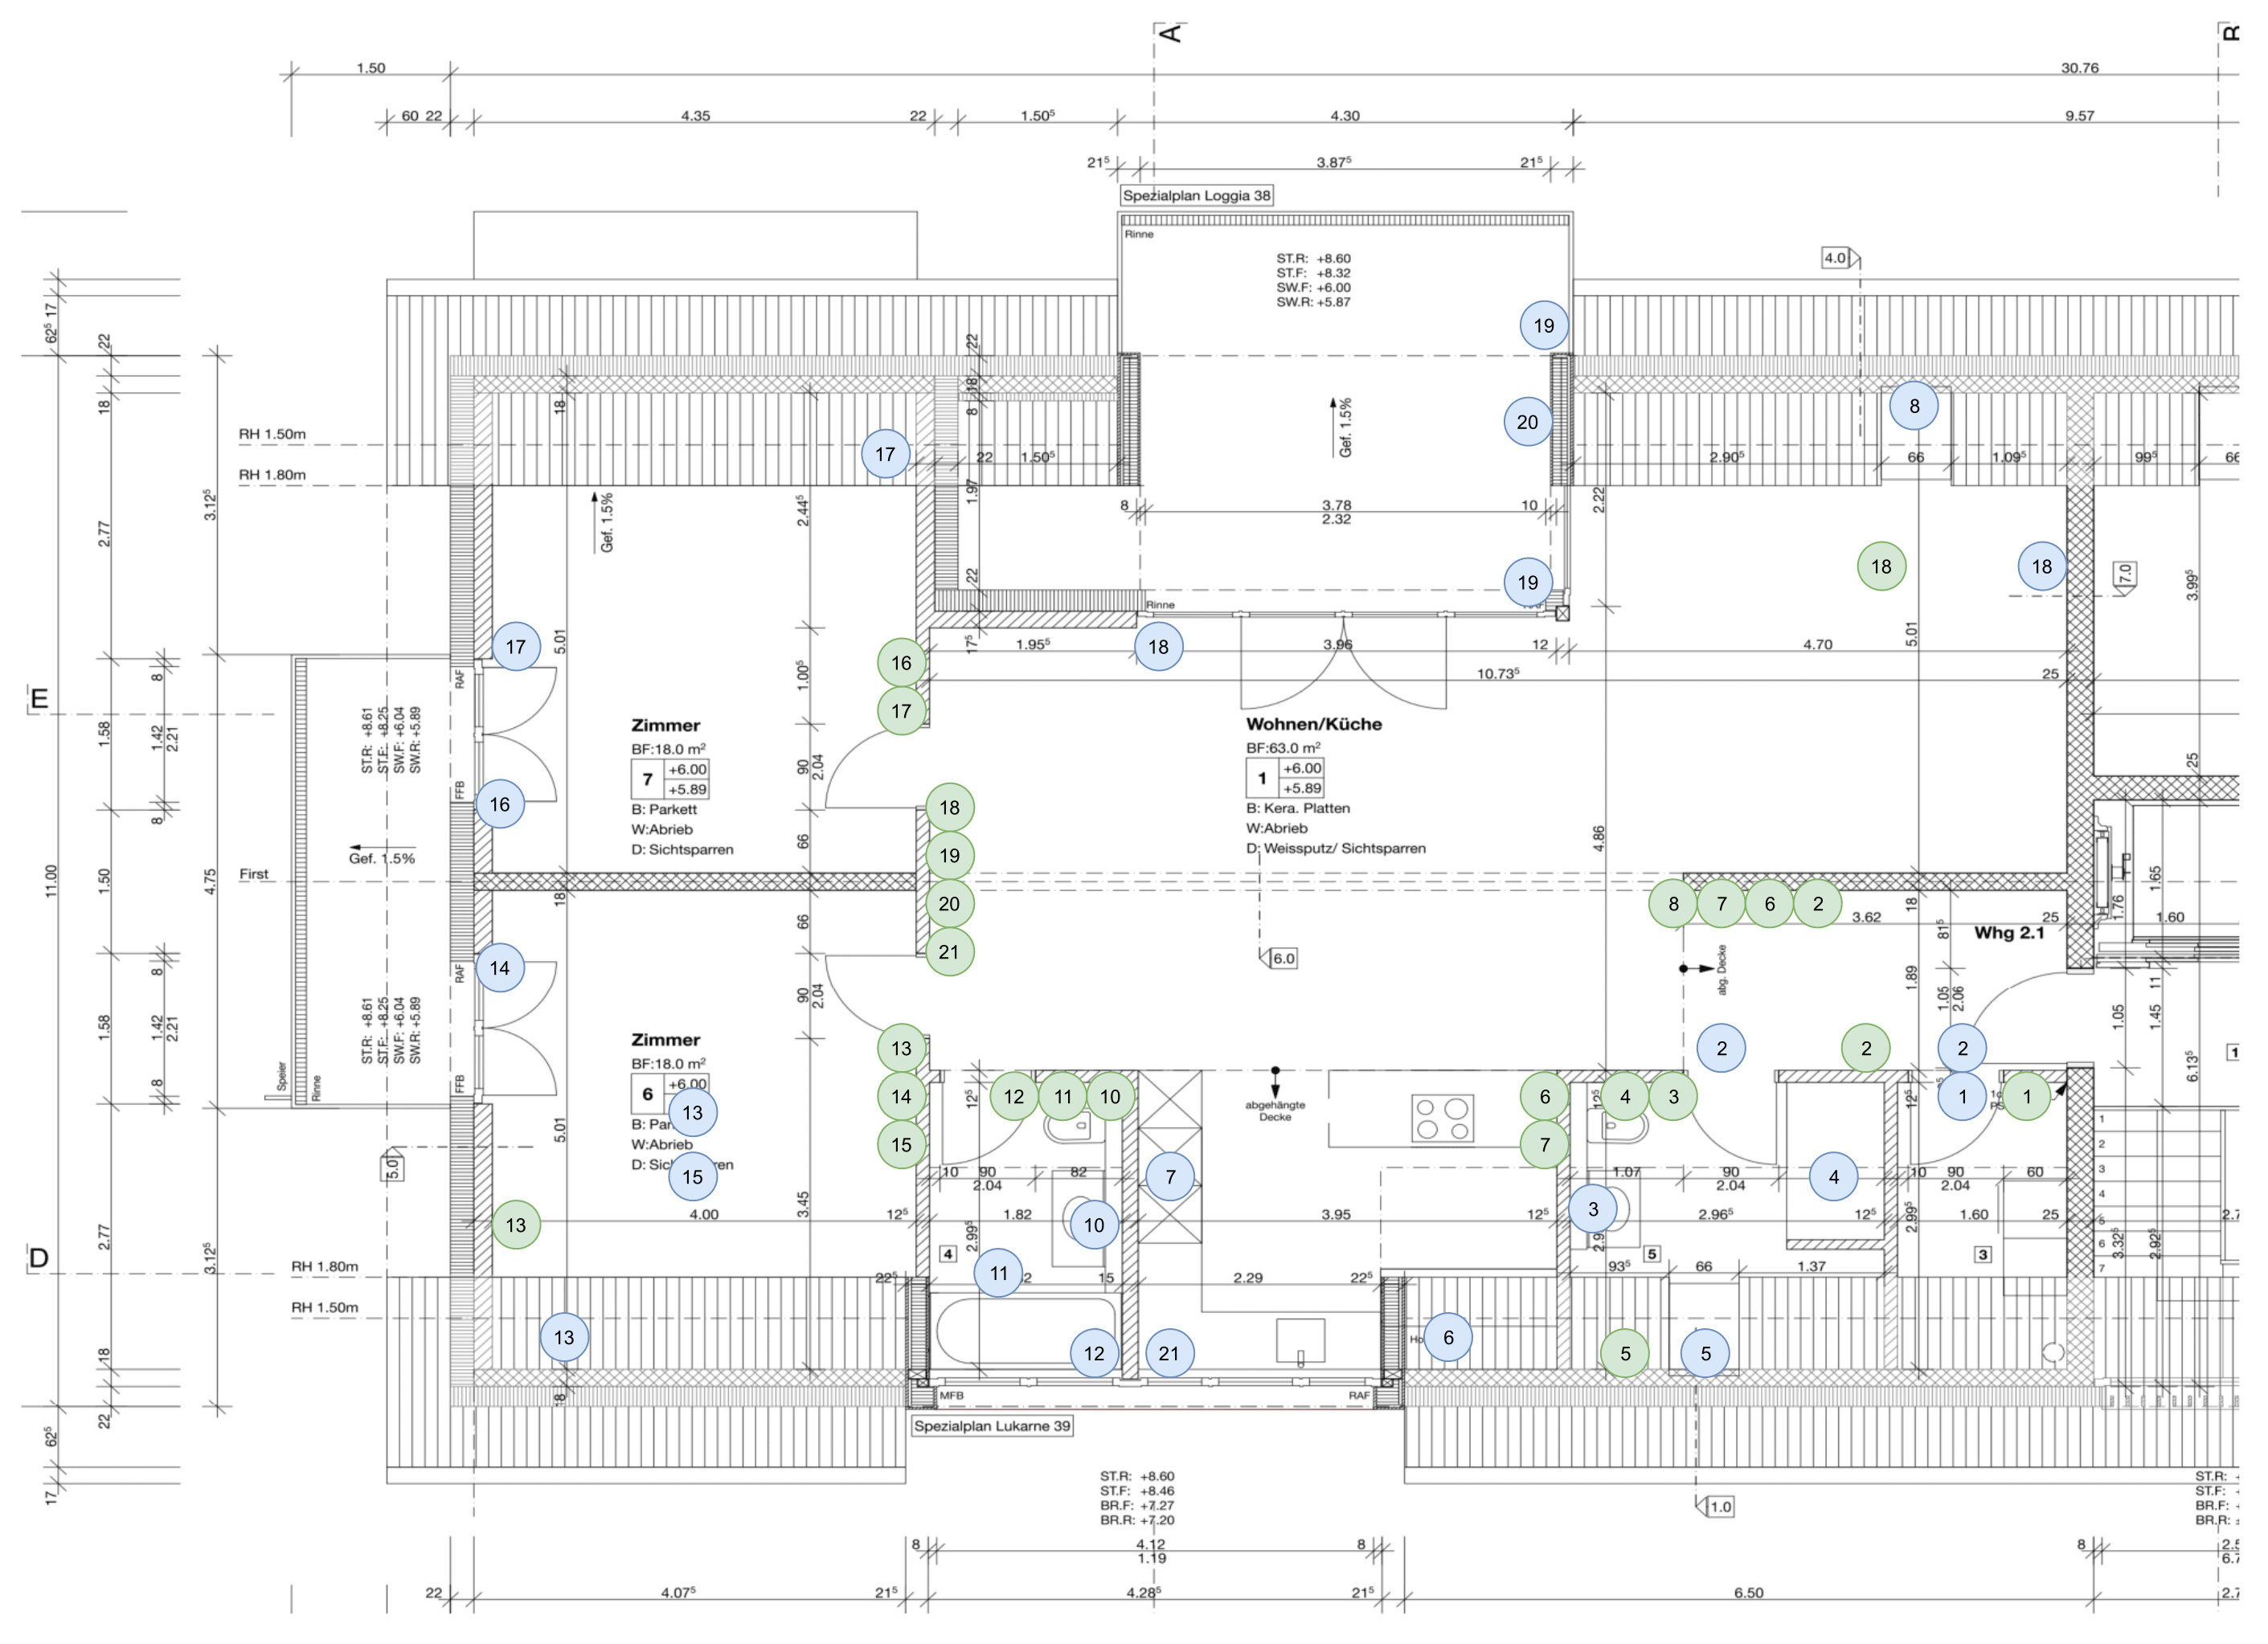
\includegraphics[width=0.6\textwidth]{graphics/Plan_Wohnung_Cyrill_Nodes_Placement.png}
	\caption{Testaufbau Wohnung}
	\label{fig:TestaufbauWohnung}
	\vspace{-100pt}
\end{wrapfigure}
Ebenfalls als Heim-Automatisierung gedacht werden die Messungen in einer Wohnung durchgeführt.

Bei der Wohnung handelt es sich um eine 3.5 Zimmer Wohnung mit einer Wohnfläche von 122 Quadratmetern. Die genauen Abmessungen sowie die Platzierung der Nodes ist in Abbildung \ref{fig:TestaufbauWohnung} zu sehen.

\vspace{30mm}
\subsection{Vergleichswerte und Messgrössen}\label{subsec:VergleichswerteundMessgrössenMesh}

\subsection{Messerwartung}
Da die Nachrichtenzustellung durch das Routing effizienter realisiert werden kann wird erwartet, dass die beiden auf dem IEEE 802.15.4 Standard aufbauenden Protokolle klare Vorteile haben werden. Hingegen könnte BT Mesh Vorteile haben bei kleiner Belastung des Netzes.

Das menschliche Auge ist in der Lage eine Verzögerung festzustellen, wenn die Latenz vom Knopfdruck bis das Licht angeht mehr als 200ms beträgt. In einer modernen Hausautomation darf natürlich keine Verzögerung wahrgenommen werden. Somit wird erwartet, dass die Latenzzeit im Schnitt unter 200ms bleiben soll. \cite{silicon_laboratories_inc_an1142_2020}